\documentclass[1p]{elsarticle_modified}
%\bibliographystyle{elsarticle-num}

%\usepackage[colorlinks]{hyperref}
%\usepackage{abbrmath_seonhwa} %\Abb, \Ascr, \Acal ,\Abf, \Afrak
\usepackage{amsfonts}
\usepackage{amssymb}
\usepackage{amsmath}
\usepackage{amsthm}
\usepackage{scalefnt}
\usepackage{amsbsy}
\usepackage{kotex}
\usepackage{caption}
\usepackage{subfig}
\usepackage{color}
\usepackage{graphicx}
\usepackage{xcolor} %% white, black, red, green, blue, cyan, magenta, yellow
\usepackage{float}
\usepackage{setspace}
\usepackage{hyperref}

\usepackage{tikz}
\usetikzlibrary{arrows}

\usepackage{multirow}
\usepackage{array} % fixed length table
\usepackage{hhline}

%%%%%%%%%%%%%%%%%%%%%
\makeatletter
\renewcommand*\env@matrix[1][\arraystretch]{%
	\edef\arraystretch{#1}%
	\hskip -\arraycolsep
	\let\@ifnextchar\new@ifnextchar
	\array{*\c@MaxMatrixCols c}}
\makeatother %https://tex.stackexchange.com/questions/14071/how-can-i-increase-the-line-spacing-in-a-matrix
%%%%%%%%%%%%%%%

\usepackage[normalem]{ulem}

\newcommand{\msout}[1]{\ifmmode\text{\sout{\ensuremath{#1}}}\else\sout{#1}\fi}
%SOURCE: \msout is \stkout macro in https://tex.stackexchange.com/questions/20609/strikeout-in-math-mode

\newcommand{\cancel}[1]{
	\ifmmode
	{\color{red}\msout{#1}}
	\else
	{\color{red}\sout{#1}}
	\fi
}

\newcommand{\add}[1]{
	{\color{blue}\uwave{#1}}
}

\newcommand{\replace}[2]{
	\ifmmode
	{\color{red}\msout{#1}}{\color{blue}\uwave{#2}}
	\else
	{\color{red}\sout{#1}}{\color{blue}\uwave{#2}}
	\fi
}

\newcommand{\Sol}{\mathcal{S}} %segment
\newcommand{\D}{D} %diagram
\newcommand{\A}{\mathcal{A}} %arc


%%%%%%%%%%%%%%%%%%%%%%%%%%%%%5 test

\def\sl{\operatorname{\textup{SL}}(2,\Cbb)}
\def\psl{\operatorname{\textup{PSL}}(2,\Cbb)}
\def\quan{\mkern 1mu \triangleright \mkern 1mu}

\theoremstyle{definition}
\newtheorem{thm}{Theorem}[section]
\newtheorem{prop}[thm]{Proposition}
\newtheorem{lem}[thm]{Lemma}
\newtheorem{ques}[thm]{Question}
\newtheorem{cor}[thm]{Corollary}
\newtheorem{defn}[thm]{Definition}
\newtheorem{exam}[thm]{Example}
\newtheorem{rmk}[thm]{Remark}
\newtheorem{alg}[thm]{Algorithm}

\newcommand{\I}{\sqrt{-1}}
\begin{document}

%\begin{frontmatter}
%
%\title{Boundary parabolic representations of knots up to 8 crossings}
%
%%% Group authors per affiliation:
%\author{Yunhi Cho} 
%\address{Department of Mathematics, University of Seoul, Seoul, Korea}
%\ead{yhcho@uos.ac.kr}
%
%
%\author{Seonhwa Kim} %\fnref{s_kim}}
%\address{Center for Geometry and Physics, Institute for Basic Science, Pohang, 37673, Korea}
%\ead{ryeona17@ibs.re.kr}
%
%\author{Hyuk Kim}
%\address{Department of Mathematical Sciences, Seoul National University, Seoul 08826, Korea}
%\ead{hyukkim@snu.ac.kr}
%
%\author{Seokbeom Yoon}
%\address{Department of Mathematical Sciences, Seoul National University, Seoul, 08826,  Korea}
%\ead{sbyoon15@snu.ac.kr}
%
%\begin{abstract}
%We find all boundary parabolic representation of knots up to 8 crossings.
%
%\end{abstract}
%\begin{keyword}
%    \MSC[2010] 57M25 
%\end{keyword}
%
%\end{frontmatter}

%\linenumbers
%\tableofcontents
%
\newcommand\colored[1]{\textcolor{white}{\rule[-0.35ex]{0.8em}{1.4ex}}\kern-0.8em\color{red} #1}%
%\newcommand\colored[1]{\textcolor{white}{ #1}\kern-2.17ex	\textcolor{white}{ #1}\kern-1.81ex	\textcolor{white}{ #1}\kern-2.15ex\color{red}#1	}

{\Large $\underline{11a_{31}~(K11a_{31})}$}

\setlength{\tabcolsep}{10pt}
\renewcommand{\arraystretch}{1.6}
\vspace{1cm}\begin{tabular}{m{100pt}>{\centering\arraybackslash}m{274pt}}
\multirow{5}{120pt}{
	\centering
	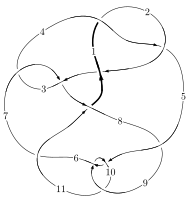
\includegraphics[width=112pt]{../../../GIT/diagram.site/Diagrams/png/280_11a_31.png}\\
\ \ \ A knot diagram\footnotemark}&
\allowdisplaybreaks
\textbf{Linearized knot diagam} \\
\cline{2-2}
 &
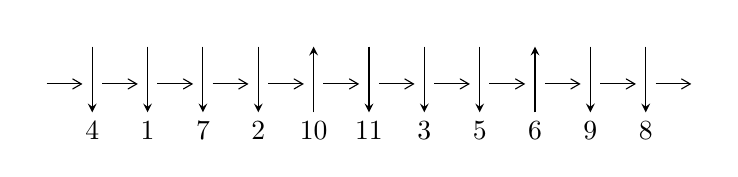
\begin{tikzpicture}[x=20pt, y=17pt]
	% nodes
	\node (C0) at (0, 0) {};
	\node (C1) at (1, 0) {};
	\node (C1U) at (1, +1) {};
	\node (C1D) at (1, -1) {4};

	\node (C2) at (2, 0) {};
	\node (C2U) at (2, +1) {};
	\node (C2D) at (2, -1) {1};

	\node (C3) at (3, 0) {};
	\node (C3U) at (3, +1) {};
	\node (C3D) at (3, -1) {7};

	\node (C4) at (4, 0) {};
	\node (C4U) at (4, +1) {};
	\node (C4D) at (4, -1) {2};

	\node (C5) at (5, 0) {};
	\node (C5U) at (5, +1) {};
	\node (C5D) at (5, -1) {10};

	\node (C6) at (6, 0) {};
	\node (C6U) at (6, +1) {};
	\node (C6D) at (6, -1) {11};

	\node (C7) at (7, 0) {};
	\node (C7U) at (7, +1) {};
	\node (C7D) at (7, -1) {3};

	\node (C8) at (8, 0) {};
	\node (C8U) at (8, +1) {};
	\node (C8D) at (8, -1) {5};

	\node (C9) at (9, 0) {};
	\node (C9U) at (9, +1) {};
	\node (C9D) at (9, -1) {6};

	\node (C10) at (10, 0) {};
	\node (C10U) at (10, +1) {};
	\node (C10D) at (10, -1) {9};

	\node (C11) at (11, 0) {};
	\node (C11U) at (11, +1) {};
	\node (C11D) at (11, -1) {8};
	\node (C12) at (12, 0) {};

	% arrows
	\draw[->,>={angle 60}]
	(C0) edge (C1) (C1) edge (C2) (C2) edge (C3) (C3) edge (C4) (C4) edge (C5) (C5) edge (C6) (C6) edge (C7) (C7) edge (C8) (C8) edge (C9) (C9) edge (C10) (C10) edge (C11) (C11) edge (C12) ;	\draw[->,>=stealth]
	(C1U) edge (C1D) (C2U) edge (C2D) (C3U) edge (C3D) (C4U) edge (C4D) (C5D) edge (C5U) (C6U) edge (C6D) (C7U) edge (C7D) (C8U) edge (C8D) (C9D) edge (C9U) (C10U) edge (C10D) (C11U) edge (C11D) ;
	\end{tikzpicture} \\
\hhline{~~} \\& 
\textbf{Solving Sequence} \\ \cline{2-2} 
 &
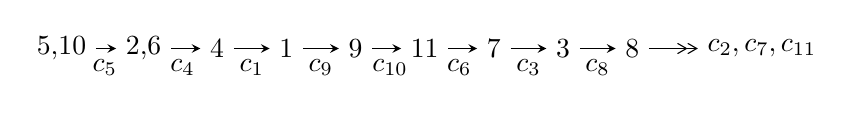
\begin{tikzpicture}[x=25pt, y=7pt]
	% node
	\node (A0) at (-1/8, 0) {5,10};
	\node (A1) at (17/16, 0) {2,6};
	\node (A2) at (17/8, 0) {4};
	\node (A3) at (25/8, 0) {1};
	\node (A4) at (33/8, 0) {9};
	\node (A5) at (41/8, 0) {11};
	\node (A6) at (49/8, 0) {7};
	\node (A7) at (57/8, 0) {3};
	\node (A8) at (65/8, 0) {8};
	\node (C1) at (1/2, -1) {$c_{5}$};
	\node (C2) at (13/8, -1) {$c_{4}$};
	\node (C3) at (21/8, -1) {$c_{1}$};
	\node (C4) at (29/8, -1) {$c_{9}$};
	\node (C5) at (37/8, -1) {$c_{10}$};
	\node (C6) at (45/8, -1) {$c_{6}$};
	\node (C7) at (53/8, -1) {$c_{3}$};
	\node (C8) at (61/8, -1) {$c_{8}$};
	\node (A9) at (10, 0) {$c_{2},c_{7},c_{11}$};

	% edge
	\draw[->,>=stealth]	
	(A0) edge (A1) (A1) edge (A2) (A2) edge (A3) (A3) edge (A4) (A4) edge (A5) (A5) edge (A6) (A6) edge (A7) (A7) edge (A8) ;
	\draw[->>,>={angle 60}]	
	(A8) edge (A9);
\end{tikzpicture} \\ 

\end{tabular} \\

\footnotetext{
The image of knot diagram is generated by the software ``\textbf{Draw programme}" developed by Andrew Bartholomew(\url{http://www.layer8.co.uk/maths/draw/index.htm\#Running-draw}), where we modified some parts for our purpose(\url{https://github.com/CATsTAILs/LinksPainter}).
}\phantom \\ \newline 
\centering \textbf{Ideals for irreducible components\footnotemark of $X_{\text{par}}$} 
 
\begin{align*}
I^u_{1}&=\langle 
- u^{65}+u^{64}+\cdots+b- u,\;- u^{65}+u^{64}+\cdots+a-1,\;u^{67}-2 u^{66}+\cdots-4 u^2+1\rangle \\
I^u_{2}&=\langle 
b+1,\;- u^3+u^2+a- u+2,\;u^5- u^4+2 u^3- u^2+u-1\rangle \\
\\
\end{align*}
\raggedright * 2 irreducible components of $\dim_{\mathbb{C}}=0$, with total 72 representations.\\
\footnotetext{All coefficients of polynomials are rational numbers. But the coefficients are sometimes approximated in decimal forms when there is not enough margin.}
\newpage
\renewcommand{\arraystretch}{1}
\centering \section*{I. $I^u_{1}= \langle - u^{65}+u^{64}+\cdots+b- u,\;- u^{65}+u^{64}+\cdots+a-1,\;u^{67}-2 u^{66}+\cdots-4 u^2+1 \rangle$}
\flushleft \textbf{(i) Arc colorings}\\
\begin{tabular}{m{7pt} m{180pt} m{7pt} m{180pt} }
\flushright $a_{5}=$&$\begin{pmatrix}1\\0\end{pmatrix}$ \\
\flushright $a_{10}=$&$\begin{pmatrix}0\\u\end{pmatrix}$ \\
\flushright $a_{2}=$&$\begin{pmatrix}u^{65}- u^{64}+\cdots-2 u+1\\u^{65}- u^{64}+\cdots-2 u^2+u\end{pmatrix}$ \\
\flushright $a_{6}=$&$\begin{pmatrix}1\\- u^2\end{pmatrix}$ \\
\flushright $a_{4}=$&$\begin{pmatrix}2 u^{65}-2 u^{64}+\cdots-2 u+2\\u^{65}- u^{64}+\cdots+5 u^3-3 u^2\end{pmatrix}$ \\
\flushright $a_{1}=$&$\begin{pmatrix}- u^{11}-2 u^9-2 u^7- u^3\\- u^{11}-3 u^9-4 u^7- u^5+u^3+u\end{pmatrix}$ \\
\flushright $a_{9}=$&$\begin{pmatrix}- u\\u^3+u\end{pmatrix}$ \\
\flushright $a_{11}=$&$\begin{pmatrix}- u^3\\u^5+u^3+u\end{pmatrix}$ \\
\flushright $a_{7}=$&$\begin{pmatrix}- u^6- u^4+1\\u^8+2 u^6+2 u^4\end{pmatrix}$ \\
\flushright $a_{3}=$&$\begin{pmatrix}- u^{63}+u^{62}+\cdots- u+1\\u^{65}- u^{64}+\cdots- u^2+u\end{pmatrix}$ \\
\flushright $a_{8}=$&$\begin{pmatrix}u^3\\u^3+u\end{pmatrix}$\\ \flushright $a_{8}=$&$\begin{pmatrix}u^3\\u^3+u\end{pmatrix}$\\&\end{tabular}
\flushleft \textbf{(ii) Obstruction class $= -1$}\\~\\
\flushleft \textbf{(iii) Cusp Shapes $= -4 u^{66}+13 u^{65}+\cdots+u-3$}\\~\\
\newpage\renewcommand{\arraystretch}{1}
\flushleft \textbf{(iv) u-Polynomials at the component}\newline \\
\begin{tabular}{m{50pt}|m{274pt}}
Crossings & \hspace{64pt}u-Polynomials at each crossing \\
\hline $$\begin{aligned}c_{1},c_{4}\end{aligned}$$&$\begin{aligned}
&u^{67}-6 u^{66}+\cdots-6 u+1
\end{aligned}$\\
\hline $$\begin{aligned}c_{2}\end{aligned}$$&$\begin{aligned}
&u^{67}+32 u^{66}+\cdots-6 u+1
\end{aligned}$\\
\hline $$\begin{aligned}c_{3},c_{7}\end{aligned}$$&$\begin{aligned}
&u^{67}+u^{66}+\cdots+96 u+32
\end{aligned}$\\
\hline $$\begin{aligned}c_{5},c_{9}\end{aligned}$$&$\begin{aligned}
&u^{67}-2 u^{66}+\cdots-4 u^2+1
\end{aligned}$\\
\hline $$\begin{aligned}c_{6},c_{8}\end{aligned}$$&$\begin{aligned}
&u^{67}+2 u^{66}+\cdots+78 u+9
\end{aligned}$\\
\hline $$\begin{aligned}c_{10}\end{aligned}$$&$\begin{aligned}
&u^{67}+36 u^{66}+\cdots+8 u-1
\end{aligned}$\\
\hline $$\begin{aligned}c_{11}\end{aligned}$$&$\begin{aligned}
&u^{67}-8 u^{66}+\cdots+2798 u+53
\end{aligned}$\\
\hline
\end{tabular}\\~\\
\newpage\renewcommand{\arraystretch}{1}
\flushleft \textbf{(v) Riley Polynomials at the component}\newline \\
\begin{tabular}{m{50pt}|m{274pt}}
Crossings & \hspace{64pt}Riley Polynomials at each crossing \\
\hline $$\begin{aligned}c_{1},c_{4}\end{aligned}$$&$\begin{aligned}
&y^{67}-32 y^{66}+\cdots-6 y-1
\end{aligned}$\\
\hline $$\begin{aligned}c_{2}\end{aligned}$$&$\begin{aligned}
&y^{67}+12 y^{66}+\cdots-266 y-1
\end{aligned}$\\
\hline $$\begin{aligned}c_{3},c_{7}\end{aligned}$$&$\begin{aligned}
&y^{67}+33 y^{66}+\cdots-14848 y-1024
\end{aligned}$\\
\hline $$\begin{aligned}c_{5},c_{9}\end{aligned}$$&$\begin{aligned}
&y^{67}+36 y^{66}+\cdots+8 y-1
\end{aligned}$\\
\hline $$\begin{aligned}c_{6},c_{8}\end{aligned}$$&$\begin{aligned}
&y^{67}-52 y^{66}+\cdots-360 y-81
\end{aligned}$\\
\hline $$\begin{aligned}c_{10}\end{aligned}$$&$\begin{aligned}
&y^{67}-8 y^{66}+\cdots+124 y-1
\end{aligned}$\\
\hline $$\begin{aligned}c_{11}\end{aligned}$$&$\begin{aligned}
&y^{67}+8 y^{66}+\cdots+6484936 y-2809
\end{aligned}$\\
\hline
\end{tabular}\\~\\
\newpage\flushleft \textbf{(vi) Complex Volumes and Cusp Shapes}
$$\begin{array}{c|c|c}  
\text{Solutions to }I^u_{1}& \I (\text{vol} + \sqrt{-1}CS) & \text{Cusp shape}\\
 \hline 
\begin{aligned}
u &= -0.564990 + 0.825170 I \\
a &= -1.000610 + 0.092379 I \\
b &= \phantom{-}0.481444 - 0.849559 I\end{aligned}
 & \phantom{-}4.87488 - 4.14687 I & -1.59935 + 4.64549 I \\ \hline\begin{aligned}
u &= -0.564990 - 0.825170 I \\
a &= -1.000610 - 0.092379 I \\
b &= \phantom{-}0.481444 + 0.849559 I\end{aligned}
 & \phantom{-}4.87488 + 4.14687 I & -1.59935 - 4.64549 I \\ \hline\begin{aligned}
u &= \phantom{-}0.511350 + 0.819428 I \\
a &= -0.40478 - 2.45910 I \\
b &= -0.887590 + 0.499549 I\end{aligned}
 & \phantom{-}0.03256 + 4.08481 I & -5.93835 - 7.04941 I \\ \hline\begin{aligned}
u &= \phantom{-}0.511350 - 0.819428 I \\
a &= -0.40478 + 2.45910 I \\
b &= -0.887590 - 0.499549 I\end{aligned}
 & \phantom{-}0.03256 - 4.08481 I & -5.93835 + 7.04941 I \\ \hline\begin{aligned}
u &= -0.569629 + 0.864915 I \\
a &= \phantom{-}1.27940 - 2.06653 I \\
b &= \phantom{-}1.098240 + 0.652944 I\end{aligned}
 & \phantom{-}3.02110 - 9.72497 I & -4.76527 + 9.27372 I \\ \hline\begin{aligned}
u &= -0.569629 - 0.864915 I \\
a &= \phantom{-}1.27940 + 2.06653 I \\
b &= \phantom{-}1.098240 - 0.652944 I\end{aligned}
 & \phantom{-}3.02110 + 9.72497 I & -4.76527 - 9.27372 I \\ \hline\begin{aligned}
u &= \phantom{-}0.246240 + 1.034280 I \\
a &= \phantom{-}0.823566 + 0.817173 I \\
b &= \phantom{-}0.575942 + 0.558676 I\end{aligned}
 & -0.281369 + 0.970663 I & \phantom{-0.000000 } 0 \\ \hline\begin{aligned}
u &= \phantom{-}0.246240 - 1.034280 I \\
a &= \phantom{-}0.823566 - 0.817173 I \\
b &= \phantom{-}0.575942 - 0.558676 I\end{aligned}
 & -0.281369 - 0.970663 I & \phantom{-0.000000 } 0 \\ \hline\begin{aligned}
u &= \phantom{-}0.119094 + 1.072640 I \\
a &= \phantom{-}2.44789 - 0.02818 I \\
b &= \phantom{-}1.039730 - 0.556055 I\end{aligned}
 & -1.77198 + 5.50921 I & \phantom{-0.000000 } 0 \\ \hline\begin{aligned}
u &= \phantom{-}0.119094 - 1.072640 I \\
a &= \phantom{-}2.44789 + 0.02818 I \\
b &= \phantom{-}1.039730 + 0.556055 I\end{aligned}
 & -1.77198 - 5.50921 I & \phantom{-0.000000 } 0\\
 \hline 
 \end{array}$$\newpage$$\begin{array}{c|c|c}  
\text{Solutions to }I^u_{1}& \I (\text{vol} + \sqrt{-1}CS) & \text{Cusp shape}\\
 \hline 
\begin{aligned}
u &= -0.052245 + 0.915458 I \\
a &= -2.62750 + 1.03290 I \\
b &= -1.058310 - 0.288428 I\end{aligned}
 & -3.49198 - 1.02780 I & -15.4724 + 0.3169 I \\ \hline\begin{aligned}
u &= -0.052245 - 0.915458 I \\
a &= -2.62750 - 1.03290 I \\
b &= -1.058310 + 0.288428 I\end{aligned}
 & -3.49198 + 1.02780 I & -15.4724 - 0.3169 I \\ \hline\begin{aligned}
u &= -0.465256 + 0.785906 I \\
a &= -0.92627 + 1.18008 I \\
b &= -1.225020 + 0.046584 I\end{aligned}
 & -1.16301 - 1.95072 I & -3.00568 + 5.39206 I \\ \hline\begin{aligned}
u &= -0.465256 - 0.785906 I \\
a &= -0.92627 - 1.18008 I \\
b &= -1.225020 - 0.046584 I\end{aligned}
 & -1.16301 + 1.95072 I & -3.00568 - 5.39206 I \\ \hline\begin{aligned}
u &= -0.574831 + 0.702829 I \\
a &= \phantom{-}0.276564 - 1.126500 I \\
b &= \phantom{-}0.534420 + 0.823507 I\end{aligned}
 & \phantom{-}5.22376 - 0.38517 I & -0.51661 + 2.40952 I \\ \hline\begin{aligned}
u &= -0.574831 - 0.702829 I \\
a &= \phantom{-}0.276564 + 1.126500 I \\
b &= \phantom{-}0.534420 - 0.823507 I\end{aligned}
 & \phantom{-}5.22376 + 0.38517 I & -0.51661 - 2.40952 I \\ \hline\begin{aligned}
u &= -0.592161 + 0.649495 I \\
a &= -0.159409 + 0.601501 I \\
b &= \phantom{-}1.063280 - 0.655308 I\end{aligned}
 & \phantom{-}3.63203 + 5.13427 I & -3.00083 - 2.99523 I \\ \hline\begin{aligned}
u &= -0.592161 - 0.649495 I \\
a &= -0.159409 - 0.601501 I \\
b &= \phantom{-}1.063280 + 0.655308 I\end{aligned}
 & \phantom{-}3.63203 - 5.13427 I & -3.00083 + 2.99523 I \\ \hline\begin{aligned}
u &= \phantom{-}0.493599 + 0.712589 I \\
a &= \phantom{-}0.989105 + 0.915694 I \\
b &= -0.797853 - 0.467895 I\end{aligned}
 & \phantom{-}0.345703 + 0.068999 I & -4.55173 - 0.43344 I \\ \hline\begin{aligned}
u &= \phantom{-}0.493599 - 0.712589 I \\
a &= \phantom{-}0.989105 - 0.915694 I \\
b &= -0.797853 + 0.467895 I\end{aligned}
 & \phantom{-}0.345703 - 0.068999 I & -4.55173 + 0.43344 I\\
 \hline 
 \end{array}$$\newpage$$\begin{array}{c|c|c}  
\text{Solutions to }I^u_{1}& \I (\text{vol} + \sqrt{-1}CS) & \text{Cusp shape}\\
 \hline 
\begin{aligned}
u &= \phantom{-}0.249006 + 0.819006 I \\
a &= \phantom{-}0.686833 + 0.149955 I \\
b &= \phantom{-}0.113095 + 0.211783 I\end{aligned}
 & -0.492874 + 1.272410 I & -5.34668 - 4.93990 I \\ \hline\begin{aligned}
u &= \phantom{-}0.249006 - 0.819006 I \\
a &= \phantom{-}0.686833 - 0.149955 I \\
b &= \phantom{-}0.113095 - 0.211783 I\end{aligned}
 & -0.492874 - 1.272410 I & -5.34668 + 4.93990 I \\ \hline\begin{aligned}
u &= \phantom{-}0.816854 + 0.158141 I \\
a &= \phantom{-}1.31512 - 1.20053 I \\
b &= \phantom{-}1.150520 + 0.623562 I\end{aligned}
 & -0.49031 - 10.48350 I & -6.68771 + 6.96472 I \\ \hline\begin{aligned}
u &= \phantom{-}0.816854 - 0.158141 I \\
a &= \phantom{-}1.31512 + 1.20053 I \\
b &= \phantom{-}1.150520 - 0.623562 I\end{aligned}
 & -0.49031 + 10.48350 I & -6.68771 - 6.96472 I \\ \hline\begin{aligned}
u &= -0.819060 + 0.039508 I \\
a &= \phantom{-}1.247840 + 0.239436 I \\
b &= \phantom{-}0.943939 + 0.369724 I\end{aligned}
 & -3.90258 - 1.39316 I & -7.44622 + 4.95368 I \\ \hline\begin{aligned}
u &= -0.819060 - 0.039508 I \\
a &= \phantom{-}1.247840 - 0.239436 I \\
b &= \phantom{-}0.943939 - 0.369724 I\end{aligned}
 & -3.90258 + 1.39316 I & -7.44622 - 4.95368 I \\ \hline\begin{aligned}
u &= \phantom{-}0.491373 + 1.074670 I \\
a &= \phantom{-}0.250948 + 0.870006 I \\
b &= \phantom{-}0.912328 + 0.663370 I\end{aligned}
 & \phantom{-}0.415223 + 0.749566 I & \phantom{-0.000000 } 0 \\ \hline\begin{aligned}
u &= \phantom{-}0.491373 - 1.074670 I \\
a &= \phantom{-}0.250948 - 0.870006 I \\
b &= \phantom{-}0.912328 - 0.663370 I\end{aligned}
 & \phantom{-}0.415223 - 0.749566 I & \phantom{-0.000000 } 0 \\ \hline\begin{aligned}
u &= \phantom{-}0.787826 + 0.169798 I \\
a &= -0.403477 + 0.028686 I \\
b &= \phantom{-}0.374311 - 0.872073 I\end{aligned}
 & \phantom{-}1.83934 - 4.96300 I & -3.50692 + 3.21590 I \\ \hline\begin{aligned}
u &= \phantom{-}0.787826 - 0.169798 I \\
a &= -0.403477 - 0.028686 I \\
b &= \phantom{-}0.374311 + 0.872073 I\end{aligned}
 & \phantom{-}1.83934 + 4.96300 I & -3.50692 - 3.21590 I\\
 \hline 
 \end{array}$$\newpage$$\begin{array}{c|c|c}  
\text{Solutions to }I^u_{1}& \I (\text{vol} + \sqrt{-1}CS) & \text{Cusp shape}\\
 \hline 
\begin{aligned}
u &= -0.771054 + 0.136932 I \\
a &= -0.93208 - 1.67887 I \\
b &= -1.010020 + 0.515425 I\end{aligned}
 & -2.81565 + 4.36823 I & -8.36975 - 4.25487 I \\ \hline\begin{aligned}
u &= -0.771054 - 0.136932 I \\
a &= -0.93208 + 1.67887 I \\
b &= -1.010020 - 0.515425 I\end{aligned}
 & -2.81565 - 4.36823 I & -8.36975 + 4.25487 I \\ \hline\begin{aligned}
u &= \phantom{-}0.506993 + 1.122470 I \\
a &= \phantom{-}1.55101 + 0.80025 I \\
b &= \phantom{-}0.704157 - 0.772274 I\end{aligned}
 & \phantom{-}1.05507 + 6.16799 I & \phantom{-0.000000 } 0 \\ \hline\begin{aligned}
u &= \phantom{-}0.506993 - 1.122470 I \\
a &= \phantom{-}1.55101 - 0.80025 I \\
b &= \phantom{-}0.704157 + 0.772274 I\end{aligned}
 & \phantom{-}1.05507 - 6.16799 I & \phantom{-0.000000 } 0 \\ \hline\begin{aligned}
u &= \phantom{-}0.751013 + 0.111032 I \\
a &= -1.48016 + 0.29513 I \\
b &= -1.254480 + 0.179113 I\end{aligned}
 & -3.63648 - 1.86851 I & -7.74469 + 3.58479 I \\ \hline\begin{aligned}
u &= \phantom{-}0.751013 - 0.111032 I \\
a &= -1.48016 - 0.29513 I \\
b &= -1.254480 - 0.179113 I\end{aligned}
 & -3.63648 + 1.86851 I & -7.74469 - 3.58479 I \\ \hline\begin{aligned}
u &= -0.423713 + 1.167870 I \\
a &= -0.210888 + 0.121533 I \\
b &= -0.351913 - 0.524199 I\end{aligned}
 & -4.77435 - 3.67797 I & \phantom{-0.000000 } 0 \\ \hline\begin{aligned}
u &= -0.423713 - 1.167870 I \\
a &= -0.210888 - 0.121533 I \\
b &= -0.351913 + 0.524199 I\end{aligned}
 & -4.77435 + 3.67797 I & \phantom{-0.000000 } 0 \\ \hline\begin{aligned}
u &= \phantom{-}0.360436 + 1.193060 I \\
a &= \phantom{-}0.685565 - 0.715503 I \\
b &= \phantom{-}0.331641 - 0.843858 I\end{aligned}
 & -2.23668 - 1.18578 I & \phantom{-0.000000 } 0 \\ \hline\begin{aligned}
u &= \phantom{-}0.360436 - 1.193060 I \\
a &= \phantom{-}0.685565 + 0.715503 I \\
b &= \phantom{-}0.331641 + 0.843858 I\end{aligned}
 & -2.23668 + 1.18578 I & \phantom{-0.000000 } 0\\
 \hline 
 \end{array}$$\newpage$$\begin{array}{c|c|c}  
\text{Solutions to }I^u_{1}& \I (\text{vol} + \sqrt{-1}CS) & \text{Cusp shape}\\
 \hline 
\begin{aligned}
u &= -0.385671 + 1.191060 I \\
a &= -1.81898 - 0.21940 I \\
b &= -1.047790 + 0.496161 I\end{aligned}
 & -6.70689 + 0.47788 I & \phantom{-0.000000 } 0 \\ \hline\begin{aligned}
u &= -0.385671 - 1.191060 I \\
a &= -1.81898 + 0.21940 I \\
b &= -1.047790 - 0.496161 I\end{aligned}
 & -6.70689 - 0.47788 I & \phantom{-0.000000 } 0 \\ \hline\begin{aligned}
u &= \phantom{-}0.402865 + 1.186580 I \\
a &= -2.97982 - 0.67442 I \\
b &= -1.251850 + 0.222499 I\end{aligned}
 & -7.37230 + 2.08523 I & \phantom{-0.000000 } 0 \\ \hline\begin{aligned}
u &= \phantom{-}0.402865 - 1.186580 I \\
a &= -2.97982 + 0.67442 I \\
b &= -1.251850 - 0.222499 I\end{aligned}
 & -7.37230 - 2.08523 I & \phantom{-0.000000 } 0 \\ \hline\begin{aligned}
u &= -0.481238 + 1.165490 I \\
a &= \phantom{-}0.648241 + 0.407995 I \\
b &= -0.501049 + 0.552756 I\end{aligned}
 & -4.35980 - 4.63647 I & \phantom{-0.000000 } 0 \\ \hline\begin{aligned}
u &= -0.481238 - 1.165490 I \\
a &= \phantom{-}0.648241 - 0.407995 I \\
b &= -0.501049 - 0.552756 I\end{aligned}
 & -4.35980 + 4.63647 I & \phantom{-0.000000 } 0 \\ \hline\begin{aligned}
u &= \phantom{-}0.363456 + 1.217370 I \\
a &= \phantom{-}2.20761 + 0.35528 I \\
b &= \phantom{-}1.152000 + 0.602107 I\end{aligned}
 & -4.67059 - 6.53918 I & \phantom{-0.000000 } 0 \\ \hline\begin{aligned}
u &= \phantom{-}0.363456 - 1.217370 I \\
a &= \phantom{-}2.20761 - 0.35528 I \\
b &= \phantom{-}1.152000 - 0.602107 I\end{aligned}
 & -4.67059 + 6.53918 I & \phantom{-0.000000 } 0 \\ \hline\begin{aligned}
u &= \phantom{-}0.678065 + 0.264736 I \\
a &= \phantom{-}0.241702 - 0.802492 I \\
b &= \phantom{-}0.639652 + 0.752359 I\end{aligned}
 & \phantom{-}3.53541 - 1.62116 I & -1.50598 + 2.39002 I \\ \hline\begin{aligned}
u &= \phantom{-}0.678065 - 0.264736 I \\
a &= \phantom{-}0.241702 + 0.802492 I \\
b &= \phantom{-}0.639652 - 0.752359 I\end{aligned}
 & \phantom{-}3.53541 + 1.62116 I & -1.50598 - 2.39002 I\\
 \hline 
 \end{array}$$\newpage$$\begin{array}{c|c|c}  
\text{Solutions to }I^u_{1}& \I (\text{vol} + \sqrt{-1}CS) & \text{Cusp shape}\\
 \hline 
\begin{aligned}
u &= \phantom{-}0.636846 + 0.349077 I \\
a &= \phantom{-}0.126882 + 0.689081 I \\
b &= \phantom{-}0.982683 - 0.638281 I\end{aligned}
 & \phantom{-}2.50124 + 3.65316 I & -3.04825 - 3.77451 I \\ \hline\begin{aligned}
u &= \phantom{-}0.636846 - 0.349077 I \\
a &= \phantom{-}0.126882 - 0.689081 I \\
b &= \phantom{-}0.982683 + 0.638281 I\end{aligned}
 & \phantom{-}2.50124 - 3.65316 I & -3.04825 + 3.77451 I \\ \hline\begin{aligned}
u &= \phantom{-}0.493300 + 1.180590 I \\
a &= -2.28193 - 1.49318 I \\
b &= -1.286340 - 0.182808 I\end{aligned}
 & -6.72971 + 6.47733 I & \phantom{-0.000000 } 0 \\ \hline\begin{aligned}
u &= \phantom{-}0.493300 - 1.180590 I \\
a &= -2.28193 + 1.49318 I \\
b &= -1.286340 + 0.182808 I\end{aligned}
 & -6.72971 - 6.47733 I & \phantom{-0.000000 } 0 \\ \hline\begin{aligned}
u &= -0.504577 + 1.182750 I \\
a &= -2.16655 + 1.99170 I \\
b &= -1.022760 - 0.541798 I\end{aligned}
 & -5.86773 - 9.08868 I & \phantom{-0.000000 } 0 \\ \hline\begin{aligned}
u &= -0.504577 - 1.182750 I \\
a &= -2.16655 - 1.99170 I \\
b &= -1.022760 + 0.541798 I\end{aligned}
 & -5.86773 + 9.08868 I & \phantom{-0.000000 } 0 \\ \hline\begin{aligned}
u &= \phantom{-}0.518615 + 1.181260 I \\
a &= -0.854148 + 0.948142 I \\
b &= \phantom{-}0.360963 + 0.899604 I\end{aligned}
 & -1.13304 + 9.79846 I & \phantom{-0.000000 } 0 \\ \hline\begin{aligned}
u &= \phantom{-}0.518615 - 1.181260 I \\
a &= -0.854148 - 0.948142 I \\
b &= \phantom{-}0.360963 - 0.899604 I\end{aligned}
 & -1.13304 - 9.79846 I & \phantom{-0.000000 } 0 \\ \hline\begin{aligned}
u &= -0.434695 + 1.222970 I \\
a &= \phantom{-}2.46804 - 0.22231 I \\
b &= \phantom{-}0.982398 + 0.369460 I\end{aligned}
 & -7.66696 - 5.81189 I & \phantom{-0.000000 } 0 \\ \hline\begin{aligned}
u &= -0.434695 - 1.222970 I \\
a &= \phantom{-}2.46804 + 0.22231 I \\
b &= \phantom{-}0.982398 - 0.369460 I\end{aligned}
 & -7.66696 + 5.81189 I & \phantom{-0.000000 } 0\\
 \hline 
 \end{array}$$\newpage$$\begin{array}{c|c|c}  
\text{Solutions to }I^u_{1}& \I (\text{vol} + \sqrt{-1}CS) & \text{Cusp shape}\\
 \hline 
\begin{aligned}
u &= \phantom{-}0.521787 + 1.193990 I \\
a &= \phantom{-}2.69334 + 1.63831 I \\
b &= \phantom{-}1.164330 - 0.627272 I\end{aligned}
 & -3.5558 + 15.4016 I & \phantom{-0.000000 } 0 \\ \hline\begin{aligned}
u &= \phantom{-}0.521787 - 1.193990 I \\
a &= \phantom{-}2.69334 - 1.63831 I \\
b &= \phantom{-}1.164330 + 0.627272 I\end{aligned}
 & -3.5558 - 15.4016 I & \phantom{-0.000000 } 0 \\ \hline\begin{aligned}
u &= -0.473515 + 1.216160 I \\
a &= \phantom{-}1.73934 - 1.24342 I \\
b &= \phantom{-}0.939042 - 0.333718 I\end{aligned}
 & -7.39058 - 3.26134 I & \phantom{-0.000000 } 0 \\ \hline\begin{aligned}
u &= -0.473515 - 1.216160 I \\
a &= \phantom{-}1.73934 + 1.24342 I \\
b &= \phantom{-}0.939042 + 0.333718 I\end{aligned}
 & -7.39058 + 3.26134 I & \phantom{-0.000000 } 0 \\ \hline\begin{aligned}
u &= -0.680235 + 0.090499 I \\
a &= \phantom{-}0.733959 + 0.447029 I \\
b &= -0.481544 - 0.437537 I\end{aligned}
 & -1.341860 + 0.241306 I & -6.37372 + 0.86588 I \\ \hline\begin{aligned}
u &= -0.680235 - 0.090499 I \\
a &= \phantom{-}0.733959 - 0.447029 I \\
b &= -0.481544 + 0.437537 I\end{aligned}
 & -1.341860 - 0.241306 I & -6.37372 - 0.86588 I \\ \hline\begin{aligned}
u &= -0.311701\phantom{ +0.000000I} \\
a &= \phantom{-}1.66731\phantom{ +0.000000I} \\
b &= -0.735196\phantom{ +0.000000I}\end{aligned}
 & -1.10322\phantom{ +0.000000I} & -8.76950\phantom{ +0.000000I}\\
 \hline 
 \end{array}$$\newpage\newpage\renewcommand{\arraystretch}{1}
\centering \section*{II. $I^u_{2}= \langle b+1,\;- u^3+u^2+a- u+2,\;u^5- u^4+2 u^3- u^2+u-1 \rangle$}
\flushleft \textbf{(i) Arc colorings}\\
\begin{tabular}{m{7pt} m{180pt} m{7pt} m{180pt} }
\flushright $a_{5}=$&$\begin{pmatrix}1\\0\end{pmatrix}$ \\
\flushright $a_{10}=$&$\begin{pmatrix}0\\u\end{pmatrix}$ \\
\flushright $a_{2}=$&$\begin{pmatrix}u^3- u^2+u-2\\-1\end{pmatrix}$ \\
\flushright $a_{6}=$&$\begin{pmatrix}1\\- u^2\end{pmatrix}$ \\
\flushright $a_{4}=$&$\begin{pmatrix}u^3- u^2+u-1\\-1\end{pmatrix}$ \\
\flushright $a_{1}=$&$\begin{pmatrix}-1\\0\end{pmatrix}$ \\
\flushright $a_{9}=$&$\begin{pmatrix}- u\\u^3+u\end{pmatrix}$ \\
\flushright $a_{11}=$&$\begin{pmatrix}- u^3\\u^4- u^3+u^2+1\end{pmatrix}$ \\
\flushright $a_{7}=$&$\begin{pmatrix}u^3\\u^3+u\end{pmatrix}$ \\
\flushright $a_{3}=$&$\begin{pmatrix}u^3- u^2+u-1\\-1\end{pmatrix}$ \\
\flushright $a_{8}=$&$\begin{pmatrix}u^3\\u^3+u\end{pmatrix}$\\ \flushright $a_{8}=$&$\begin{pmatrix}u^3\\u^3+u\end{pmatrix}$\\&\end{tabular}
\flushleft \textbf{(ii) Obstruction class $= 1$}\\~\\
\flushleft \textbf{(iii) Cusp Shapes $= 2 u^4+u^3+2 u-12$}\\~\\
\newpage\renewcommand{\arraystretch}{1}
\flushleft \textbf{(iv) u-Polynomials at the component}\newline \\
\begin{tabular}{m{50pt}|m{274pt}}
Crossings & \hspace{64pt}u-Polynomials at each crossing \\
\hline $$\begin{aligned}c_{1}\end{aligned}$$&$\begin{aligned}
&(u-1)^5
\end{aligned}$\\
\hline $$\begin{aligned}c_{2},c_{4}\end{aligned}$$&$\begin{aligned}
&(u+1)^5
\end{aligned}$\\
\hline $$\begin{aligned}c_{3},c_{7}\end{aligned}$$&$\begin{aligned}
&u^5
\end{aligned}$\\
\hline $$\begin{aligned}c_{5}\end{aligned}$$&$\begin{aligned}
&u^5- u^4+2 u^3- u^2+u-1
\end{aligned}$\\
\hline $$\begin{aligned}c_{6}\end{aligned}$$&$\begin{aligned}
&u^5+u^4-2 u^3- u^2+u-1
\end{aligned}$\\
\hline $$\begin{aligned}c_{8},c_{11}\end{aligned}$$&$\begin{aligned}
&u^5- u^4-2 u^3+u^2+u+1
\end{aligned}$\\
\hline $$\begin{aligned}c_{9}\end{aligned}$$&$\begin{aligned}
&u^5+u^4+2 u^3+u^2+u+1
\end{aligned}$\\
\hline $$\begin{aligned}c_{10}\end{aligned}$$&$\begin{aligned}
&u^5+3 u^4+4 u^3+u^2- u-1
\end{aligned}$\\
\hline
\end{tabular}\\~\\
\newpage\renewcommand{\arraystretch}{1}
\flushleft \textbf{(v) Riley Polynomials at the component}\newline \\
\begin{tabular}{m{50pt}|m{274pt}}
Crossings & \hspace{64pt}Riley Polynomials at each crossing \\
\hline $$\begin{aligned}c_{1},c_{2},c_{4}\end{aligned}$$&$\begin{aligned}
&(y-1)^5
\end{aligned}$\\
\hline $$\begin{aligned}c_{3},c_{7}\end{aligned}$$&$\begin{aligned}
&y^5
\end{aligned}$\\
\hline $$\begin{aligned}c_{5},c_{9}\end{aligned}$$&$\begin{aligned}
&y^5+3 y^4+4 y^3+y^2- y-1
\end{aligned}$\\
\hline $$\begin{aligned}c_{6},c_{8},c_{11}\end{aligned}$$&$\begin{aligned}
&y^5-5 y^4+8 y^3-3 y^2- y-1
\end{aligned}$\\
\hline $$\begin{aligned}c_{10}\end{aligned}$$&$\begin{aligned}
&y^5- y^4+8 y^3-3 y^2+3 y-1
\end{aligned}$\\
\hline
\end{tabular}\\~\\
\newpage\flushleft \textbf{(vi) Complex Volumes and Cusp Shapes}
$$\begin{array}{c|c|c}  
\text{Solutions to }I^u_{2}& \I (\text{vol} + \sqrt{-1}CS) & \text{Cusp shape}\\
 \hline 
\begin{aligned}
u &= -0.339110 + 0.822375 I \\
a &= -1.12878 + 1.10766 I \\
b &= -1.00000\phantom{ +0.000000I}\end{aligned}
 & -1.97403 - 1.53058 I & -12.02124 + 2.62456 I \\ \hline\begin{aligned}
u &= -0.339110 - 0.822375 I \\
a &= -1.12878 - 1.10766 I \\
b &= -1.00000\phantom{ +0.000000I}\end{aligned}
 & -1.97403 + 1.53058 I & -12.02124 - 2.62456 I \\ \hline\begin{aligned}
u &= \phantom{-}0.766826\phantom{ +0.000000I} \\
a &= -1.37029\phantom{ +0.000000I} \\
b &= -1.00000\phantom{ +0.000000I}\end{aligned}
 & -4.04602\phantom{ +0.000000I} & -9.32390\phantom{ +0.000000I} \\ \hline\begin{aligned}
u &= \phantom{-}0.455697 + 1.200150 I \\
a &= -2.18608 - 0.87465 I \\
b &= -1.00000\phantom{ +0.000000I}\end{aligned}
 & -7.51750 + 4.40083 I & -12.31681 - 3.97407 I \\ \hline\begin{aligned}
u &= \phantom{-}0.455697 - 1.200150 I \\
a &= -2.18608 + 0.87465 I \\
b &= -1.00000\phantom{ +0.000000I}\end{aligned}
 & -7.51750 - 4.40083 I & -12.31681 + 3.97407 I\\
 \hline 
 \end{array}$$\newpage
\newpage\renewcommand{\arraystretch}{1}
\centering \section*{ III. u-Polynomials}
\begin{tabular}{m{50pt}|m{274pt}}
Crossings & \hspace{64pt}u-Polynomials at each crossing \\
\hline $$\begin{aligned}c_{1}\end{aligned}$$&$\begin{aligned}
&((u-1)^5)(u^{67}-6 u^{66}+\cdots-6 u+1)
\end{aligned}$\\
\hline $$\begin{aligned}c_{2}\end{aligned}$$&$\begin{aligned}
&((u+1)^5)(u^{67}+32 u^{66}+\cdots-6 u+1)
\end{aligned}$\\
\hline $$\begin{aligned}c_{3},c_{7}\end{aligned}$$&$\begin{aligned}
&u^5(u^{67}+u^{66}+\cdots+96 u+32)
\end{aligned}$\\
\hline $$\begin{aligned}c_{4}\end{aligned}$$&$\begin{aligned}
&((u+1)^5)(u^{67}-6 u^{66}+\cdots-6 u+1)
\end{aligned}$\\
\hline $$\begin{aligned}c_{5}\end{aligned}$$&$\begin{aligned}
&(u^5- u^4+2 u^3- u^2+u-1)(u^{67}-2 u^{66}+\cdots-4 u^2+1)
\end{aligned}$\\
\hline $$\begin{aligned}c_{6}\end{aligned}$$&$\begin{aligned}
&(u^5+u^4-2 u^3- u^2+u-1)(u^{67}+2 u^{66}+\cdots+78 u+9)
\end{aligned}$\\
\hline $$\begin{aligned}c_{8}\end{aligned}$$&$\begin{aligned}
&(u^5- u^4-2 u^3+u^2+u+1)(u^{67}+2 u^{66}+\cdots+78 u+9)
\end{aligned}$\\
\hline $$\begin{aligned}c_{9}\end{aligned}$$&$\begin{aligned}
&(u^5+u^4+2 u^3+u^2+u+1)(u^{67}-2 u^{66}+\cdots-4 u^2+1)
\end{aligned}$\\
\hline $$\begin{aligned}c_{10}\end{aligned}$$&$\begin{aligned}
&(u^5+3 u^4+4 u^3+u^2- u-1)(u^{67}+36 u^{66}+\cdots+8 u-1)
\end{aligned}$\\
\hline $$\begin{aligned}c_{11}\end{aligned}$$&$\begin{aligned}
&(u^5- u^4-2 u^3+u^2+u+1)(u^{67}-8 u^{66}+\cdots+2798 u+53)
\end{aligned}$\\
\hline
\end{tabular}\newpage\renewcommand{\arraystretch}{1}
\centering \section*{ IV. Riley Polynomials}
\begin{tabular}{m{50pt}|m{274pt}}
Crossings & \hspace{64pt}Riley Polynomials at each crossing \\
\hline $$\begin{aligned}c_{1},c_{4}\end{aligned}$$&$\begin{aligned}
&((y-1)^5)(y^{67}-32 y^{66}+\cdots-6 y-1)
\end{aligned}$\\
\hline $$\begin{aligned}c_{2}\end{aligned}$$&$\begin{aligned}
&((y-1)^5)(y^{67}+12 y^{66}+\cdots-266 y-1)
\end{aligned}$\\
\hline $$\begin{aligned}c_{3},c_{7}\end{aligned}$$&$\begin{aligned}
&y^5(y^{67}+33 y^{66}+\cdots-14848 y-1024)
\end{aligned}$\\
\hline $$\begin{aligned}c_{5},c_{9}\end{aligned}$$&$\begin{aligned}
&(y^5+3 y^4+4 y^3+y^2- y-1)(y^{67}+36 y^{66}+\cdots+8 y-1)
\end{aligned}$\\
\hline $$\begin{aligned}c_{6},c_{8}\end{aligned}$$&$\begin{aligned}
&(y^5-5 y^4+8 y^3-3 y^2- y-1)(y^{67}-52 y^{66}+\cdots-360 y-81)
\end{aligned}$\\
\hline $$\begin{aligned}c_{10}\end{aligned}$$&$\begin{aligned}
&(y^5- y^4+8 y^3-3 y^2+3 y-1)(y^{67}-8 y^{66}+\cdots+124 y-1)
\end{aligned}$\\
\hline $$\begin{aligned}c_{11}\end{aligned}$$&$\begin{aligned}
&(y^5-5 y^4+8 y^3-3 y^2- y-1)(y^{67}+8 y^{66}+\cdots+6484936 y-2809)
\end{aligned}$\\
\hline
\end{tabular}
\vskip 2pc
\end{document}